%%%%%%%%%%%%%%%%%%%%%%%%%%%%%%%%%%%%%%%%%
% Beamer Presentation

\documentclass{beamer}
\mode<presentation> {
% Theme
\usetheme{metropolis}
%\setbeamertemplate{footline} % To remove the footer line in all slides uncomment this line
%\setbeamertemplate{footline}[page number] % To replace the footer line in all slides with a simple slide count uncomment this line
%\setbeamertemplate{navigation symbols}{} % To remove the navigation symbols from the bottom of all slides uncomment this line
}

%Packages
\usepackage{graphicx} % Allows including images
\usepackage{booktabs} % Allows the use of \toprule, \midrule and \bottomrule in tables
%\usepackage{cite}
\usepackage[numbers]{natbib} % For bibliography
\usepackage{multirow}
\usepackage{hyperref}
%\usetheme{Warsaw}
\usepackage[absolute,overlay]{textpos}
\usepackage{xcolor}


% Colors
%\definecolor{Red}{rgb}{0.7,0,0}
%\definecolor{Blue}{rgb}{0,0,0.8}

% Prepare title and TOC
\title[Short title]{Introduction to R} 
\author{Marco Chiapello} 
\institute[Center for Proteomics] 
{
Center for Proteomics\\
University of Cambridge \\ 
\medskip
\textit{mc983@cam.ac.uk} 
}
\date{\today} 

%\AtBeginSection[]
%{
%\begin{frame}<beamer>
%\frametitle{Overview}
%\tableofcontents[currentsection]
%\end{frame}
%}


%-------------------------------------------
% MAIN DOCUMENT
%-------------------------------------------
\usepackage{Sweave}
\begin{document}
\Sconcordance{concordance:Rbasic_Day1.tex:Rbasic_Day1.Rnw:%
1 54 1 1 0 184 1 1 2 6 0 1 1 5 0 1 1 5 0 1 1 6 0 1 2 9 1 1 2 7 0 1 2 11 %
1 1 2 1 0 1 1 6 0 1 2 2 1 1 2 1 0 1 1 6 0 1 2 7 1 1 2 7 0 1 2 2 1 1 2 6 %
0 2 1 6 0 1 2 8 1 1 2 6 0 1 1 5 0 1 1 6 0 1 2 8 1 1 2 1 0 1 1 6 0 1 2 %
15 1 1 2 7 0 1 2 8 1 1 2 7 0 1 2 10 1 1 2 7 0 1 2 20 1 1 2 7 0 1 2 9 1 %
1 2 7 0 1 2 9 1 1 2 1 0 1 1 6 0 1 2 9 1 1 2 7 0 1 2 14 1 1 2 7 0 1 2 7 %
1 1 2 7 0 1 2 3 1 1 2 7 0 1 2 10 1 1 3 8 0 1 2 11 1 1 3 8 0 1 2 9 1 1 3 %
8 0 1 2 18 1 1 2 7 0 1 2 9 1 1 2 6 0 1 1 6 0 1 2 9 1 1 2 6 0 1 1 6 0 1 %
2 9 1 1 2 1 0 1 1 5 0 1 1 5 0 1 2 7 0 1 2 7 1 1 2 1 0 2 1 6 0 1 2 8 1 1 %
2 1 0 1 1 6 0 1 2 3 1 1 2 6 0 1 1 6 0 1 2 9 1 1 2 1 0 1 1 6 0 1 2 5 1 1 %
2 1 0 1 1 5 0 2 1 7 0 1 2 57 1 1 2 1 0 1 1 1 2 1 0 2 1 3 0 1 2 5 1 1 2 %
1 0 1 1 7 0 1 2 12 1 1 2 1 0 1 1 7 0 1 2 5 1 1 2 7 0 1 1 7 0 1 2 12 1 1 %
2 1 0 1 1 6 0 1 2 105 1 1 13 1 2 17 0 1 2 10 1 1 2 1 0 1 1 3 0 1 2 6 1 %
1 3 2 0 1 2 4 0 1 2 6 1 1 2 4 0 1 2 12 1 1 2 7 0 1 2 7 1 1 2 6 0 1 1 5 %
0 1 1 5 0 1 1 6 0 1 2 18 1 1 2 7 0 1 1 7 0 1 2 18 1 1 3 2 0 1 1 16 0 1 %
2 5 1 1 2 7 0 1 2 14 1 1 3 2 0 1 1 7 0 1 2 5 1 1 4 3 0 1 1 7 0 1 2 13 1 %
1 2 1 0 1 1 11 0 2 2 1 0 1 1 8 0 1 2 18 1 1 2 1 0 4 1 9 0 1 2 2 1 1 2 7 %
0 1 2 19 1 1 2 8 0 1 2 2 1 1 2 8 0 2 2 9 0 1 2 16 1 1 2 6 0 1 1 6 0 1 2 %
18 1 1 2 1 0 1 1 5 0 1 1 5 0 2 1 5 0 1 1 5 0 1 1 5 0 1 1 6 0 1 2 68 1 1 %
2 1 0 6 1 16 0 1 2 18 1 1 2 7 0 1 2 8 1 1 2 1 0 1 1 5 0 2 1 10 0 1 1 6 %
0 1 2 1 1 1 2 6 0 1 1 5 0 1 1 6 0 1 2 16 1 1 2 7 0 1 2 8 1 1 2 10 0 1 2 %
8 1 1 2 7 0 1 2 16 1 1 2 1 0 1 1 7 0 1 2 8 1 1 2 1 0 1 1 6 0 1 1 5 0 1 %
1 7 0 1 2 126 1 1 2 1 0 1 1 5 0 2 1 5 0 1 1 3 0 1 2 13 1 1 2 1 0 1 1 9 %
0 1 1 505 0 1 2 39 1 1 2 1 0 2 1 505 0 1 2 23 1 1 2 1 0 1 1 6 0 1 2 113 %
1 1 2 4 0 1 2 212 1}

\newlength{\fancyvrbtopsep}
\newlength{\fancyvrbpartopsep}
\makeatletter
\FV@AddToHook{\FV@ListParameterHook}{\topsep=\fancyvrbtopsep\partopsep=\fancyvrbpartopsep}
\makeatother
\setlength{\fancyvrbtopsep}{-3pt}
\setlength{\fancyvrbpartopsep}{-3pt}

%-------------------------------------------
% TITLE PAGE
%-------------------------------------------
\begin{frame}
	\titlepage 
\end{frame}

%-------------------------------------------
% TABLE OF CONTENTS
%-------------------------------------------
\begin{frame}{Overview}
	\small
	\tableofcontents
\end{frame}

%----------------------------------------------------------------------------------------
%	PRESENTATION SLIDES
%----------------------------------------------------------------------------------------

%-------------------
% INTRODUCTION
%-------------------
\section{Introduction}

%%%%%%% 
\begin{frame}
	\frametitle{What R is?}
	\Large The \texttt{R} Project for Statistical Computing
	\begin{itemize}
		\small
		\item \texttt{R} is a free software environment for statistical computing and graphics
		\item Open source and cross platform (UNIX platforms, Windows and MacOS)
		\item Extensive graphics capabilities
		\item Diverse range of add-on packages
		\item Active community of developers
		\item Thorough documentation
	\end{itemize}
\end{frame}

%%%%%%% 
\begin{frame}
	\frametitle{What R is?}
        \Large The \texttt{R} Project for Statistical Computing\\
	\small You can find \texttt{R} here:
	\url{https://www.r-project.org}\\
	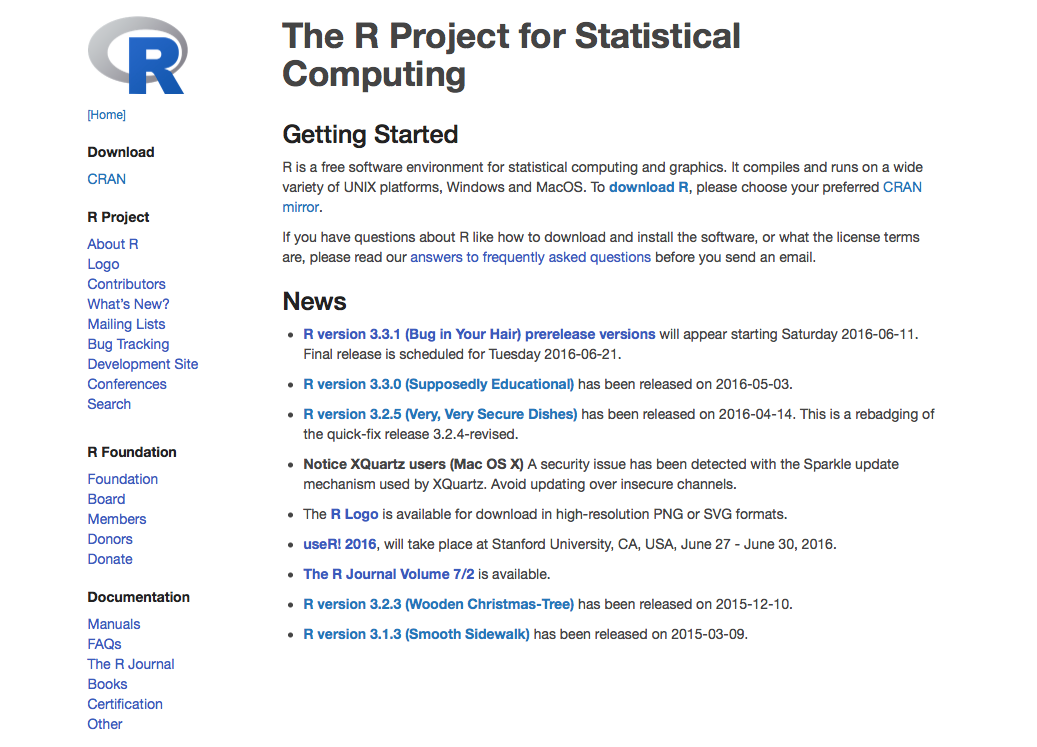
\includegraphics[scale=0.25]{figures/R-project.png}
\end{frame}

%%%%%%% 
\begin{frame}
	\frametitle{What R is?}
        \Large The \texttt{R} Project for Statistical Computing\\
	\begin{itemize}
		\small
		\item R version 3.3.1 (released 2016-06-21)
		\item Currently, the CRAN {\tiny(Comprehensive R Archive Network)} package repository features 8609 available packages
			\begin{itemize}
				\item \tiny \url{https://cran.r-project.org/web/packages/available_packages_by_name.html}
			\end{itemize}
		\item Currently, the Bioconductor repository features 1211 available packages
			\begin{itemize}
				\item \tiny \url{http://www.bioconductor.org}
			\end{itemize}
		\item Executed using command line, or a graphical user interface (GUI)
		\item On this course, we use the RStudio GUI
			\begin{itemize}
				\item \tiny \url{www.rstudio.com}
			\end{itemize}
	\end{itemize}
\end{frame}

%%%%%%% 
\begin{frame}[fragile]
	\frametitle{Getting started}
        \begin{itemize}
          \item \texttt{R} is a program which, once installed on your system, can be launched and is immediately ready to take input directly from the user
          \item There are two ways to launch R:
            \begin{enumerate}
              \small
              \item From the command line (particularly useful if you're quite familiar with Linux)
              \item As an application called RStudio (very good for beginners)
            \end{enumerate}
        \end{itemize}
\end{frame}

%%%%%%% 
\begin{frame}
	\frametitle{Launch R}
  \texttt{R} can be launched in 2 ways:
  \begin{enumerate}
    \item From command line
      \begin{itemize}
        \item To start \texttt{R} you need to enter the console (also called terminal or shell)
        \item To start \texttt{R}, at the prompt simply type: \Large \texttt{R}
      \end{itemize}
    \item Using RStudio
      \begin{itemize}
          \item To launch RStudio, find the RStudio icon and double-click
        \end{itemize}
  \end{enumerate}
\end{frame}

%%%%%%% 
\begin{frame}
	\frametitle{RStudio}
	Since we will use RStudio in this course, let's have a look of the program\\
	\centering 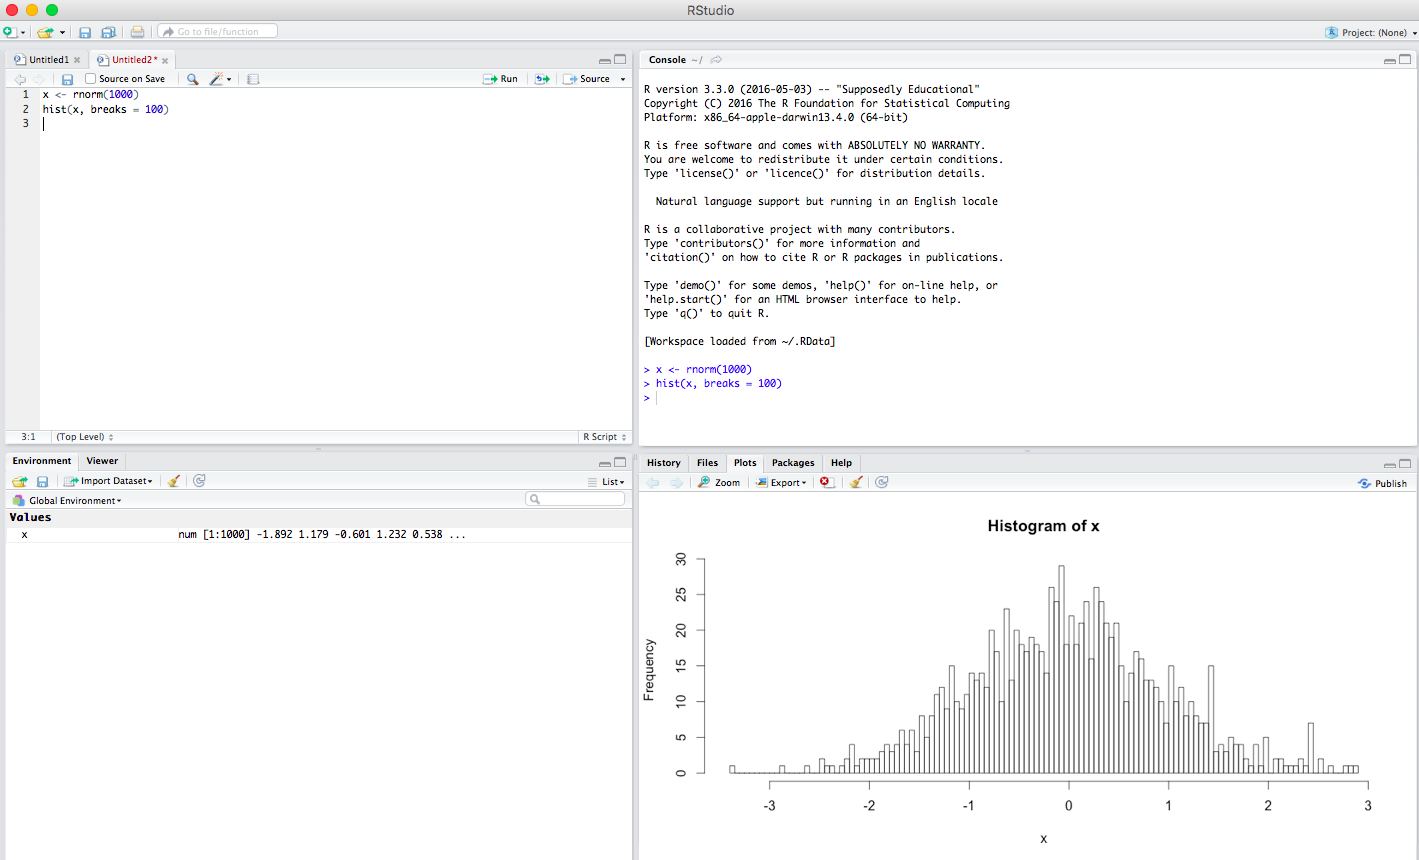
\includegraphics[scale=1.4]{figures/Rstudio_overview.png}
\end{frame}

%%%%%%% 
\begin{frame}
	\frametitle{RStudio}
	\textbf{R console}\\
	\vspace{20pt}
	\centering 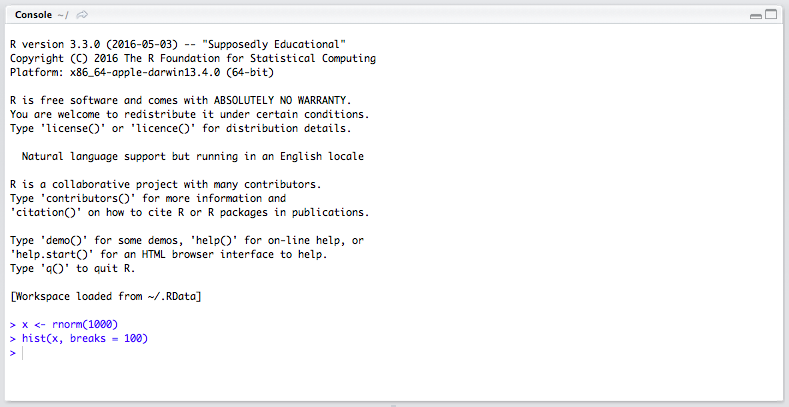
\includegraphics[width=11cm]{figures/RStudio_console.png}\\
	\small It is the place where you can interactively run R commands
\end{frame}

%%%%%%% 
\begin{frame}
	\frametitle{RStudio}
	\textbf{Source editor for R scripts}\\
	\vspace{20pt}
	\centering 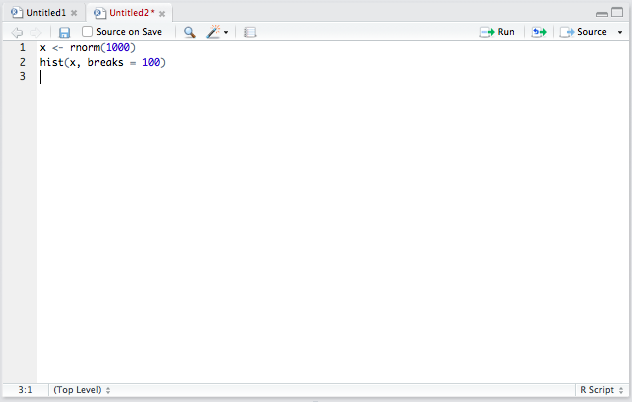
\includegraphics[width=10cm]{figures/RStudio_script.png}\\
	\small It is the place where you can write your scripts
\end{frame}

%%%%%%% 
\begin{frame}
	\frametitle{RStudio}
	\textbf{Workspace}\\
	\vspace{16pt}
	\centering 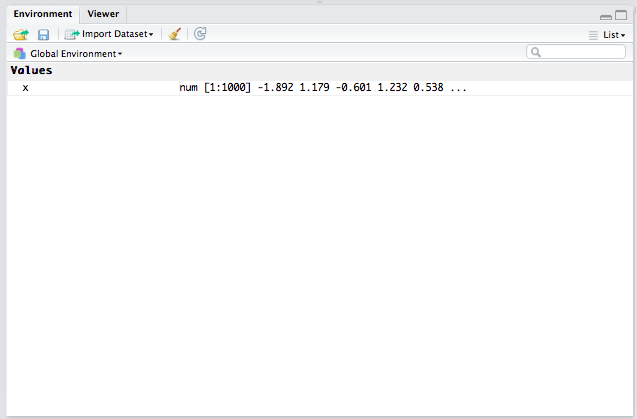
\includegraphics[width=10cm]{figures/RStudio_environment.png}\\
	\small It is the place where you can view object in the global environment
\end{frame}

%%%%%%% 
\begin{frame}
	\frametitle{RStudio}
	\textbf{Plot pannel}\\
	\vspace{20pt}
	\centering 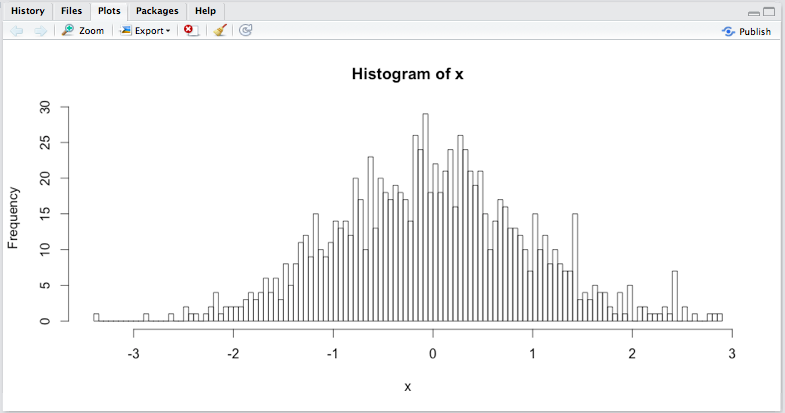
\includegraphics[width=10cm]{figures/RStudio_plot.png}\\
	\small It is the place where you can view your plots
\end{frame}

%%%%%%% 
\begin{frame}
	\frametitle{RStudio}
	\textbf{R help}\\
	\vspace{20pt}
	\centering 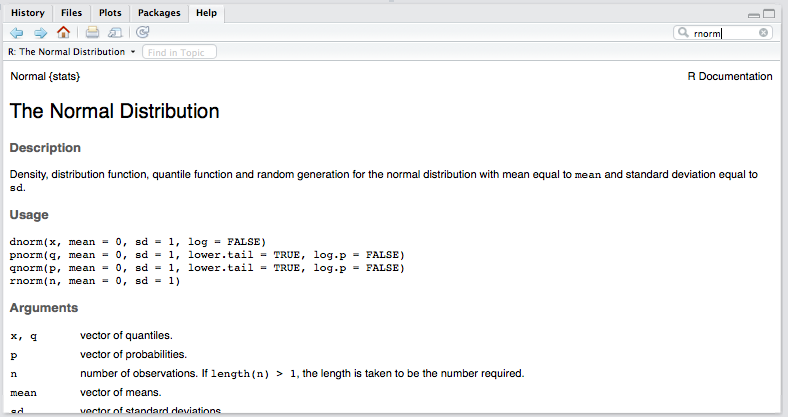
\includegraphics[width=10cm]{figures/RStudio_help.png}\\
	\small It is the place where you can find help
\end{frame}

%%%%%%% 
\begin{frame}
	\frametitle{RStudio}
	The GUI is divided into 4 main sub-windows\\
	These sub-windows are customizable\\
	\vspace{10pt}
	\centering 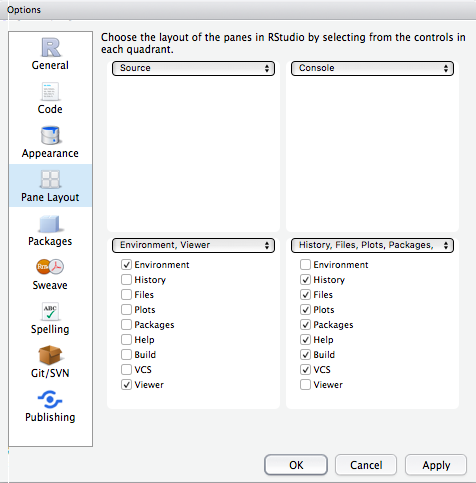
\includegraphics[width=7cm]{figures/RStudio_option.png}
\end{frame}

%%%%%%%%%%%%%%%%%%%%%%%%%%%%%%%%%%%%%%%%%%%%%%%%%%%%%%%%%%%%%%%%%%%%%%
%%%%%%%%%%%%%%%%%%%%%%%%%%%%%%%%%%%%%%%%%%%%%%%%%%%%%%%%%%%%%%%%%%%%%%
\section{Basic concepts in R}

%%%%%%% 
\begin{frame}[fragile]{prova}
	\frametitle{Numbers}
	The command line can be used as a calculator
\rule{\textwidth}{0.4pt}
\begin{Schunk}
\begin{Sinput}
> 5 + 7 
\end{Sinput}
\begin{Soutput}
[1] 12
\end{Soutput}
\begin{Sinput}
> 5 - 7
\end{Sinput}
\begin{Soutput}
[1] -2
\end{Soutput}
\begin{Sinput}
> 5 * 7
\end{Sinput}
\begin{Soutput}
[1] 35
\end{Soutput}
\begin{Sinput}
> 5 / 7
\end{Sinput}
\begin{Soutput}
[1] 0.7142857
\end{Soutput}
\end{Schunk}
\rule{\textwidth}{0.4pt}
\vspace{5pt}
\small Note: The number in the square brackets is an indicator of the position in the output
\end{frame}

%%%%%%% 
\begin{frame}[fragile]{prova}
	\frametitle{Numbers}
	You can solve simple or complex calculations 
	\rule{\textwidth}{0.4pt}
\begin{Schunk}
\begin{Sinput}
> (((20/5)^2)-((5+1/3+4/5-10)*(2-34))-20)
\end{Sinput}
\begin{Soutput}
[1] -127.7333
\end{Soutput}
\end{Schunk}
\rule{\textwidth}{0.4pt}
\vspace{20pt}
\Large But, of course, \texttt{R} is not a calculator
\end{frame}

%%%%%%% 
\begin{frame}[fragile]
	\frametitle{Variables}
	A \textbf{variable} is a letter or word which takes (or contains) a value. We use the assignment 'operator', <-\\
	\vspace{10pt}
	- We can assign a number to a variable
	\rule{\textwidth}{0.4pt}
\begin{Schunk}
\begin{Sinput}
> x <- 5
> x
\end{Sinput}
\begin{Soutput}
[1] 5
\end{Soutput}
\end{Schunk}
 \rule{\textwidth}{0.4pt}
 - We can assign the result of an operation to a variable
 \rule{\textwidth}{0.4pt}
\begin{Schunk}
\begin{Sinput}
> y <- 5 + 7
> y
\end{Sinput}
\begin{Soutput}
[1] 12
\end{Soutput}
\end{Schunk}
\rule{\textwidth}{0.4pt}
\end{frame}

%%%%%%% 
\begin{frame}[fragile]
	\frametitle{Variables}
	- We can assign use the variables to perform calculation
	\rule{\textwidth}{0.4pt}
\begin{Schunk}
\begin{Sinput}
> x + y
\end{Sinput}
\begin{Soutput}
[1] 17
\end{Soutput}
\end{Schunk}
 \rule{\textwidth}{0.4pt}
 - We can assign the change the content of the variable
 \rule{\textwidth}{0.4pt}
\begin{Schunk}
\begin{Sinput}
> x
\end{Sinput}
\begin{Soutput}
[1] 5
\end{Soutput}
\begin{Sinput}
> x <- x - y
> x
\end{Sinput}
\begin{Soutput}
[1] -7
\end{Soutput}
\end{Schunk}
\rule{\textwidth}{0.4pt}
\end{frame}

%%%%%%% 
\begin{frame}[fragile]
	\frametitle{Function}
	\textbf{Functions} in \texttt{R} perform operations on arguments (the input(s) to the function). \\ Arguments are always contained in parentheses, i.e. curved brackets (), separated by commas.
	\vspace{10pt}
	
\begin{Schunk}
\begin{Sinput}
> sum(3, 4, 5, 6)
\end{Sinput}
\begin{Soutput}
[1] 18
\end{Soutput}
\begin{Sinput}
> max(3, 4, 5, 6)
\end{Sinput}
\begin{Soutput}
[1] 6
\end{Soutput}
\begin{Sinput}
> min(3, 4, 5, 6)
\end{Sinput}
\begin{Soutput}
[1] 3
\end{Soutput}
\end{Schunk}

\end{frame}

%%%%%%% 
\begin{frame}[fragile]
	\frametitle{Function extention}
	\texttt{R} contains a lot of pre-builtin functions, but through the so called \textit{packages} is possible extend the \texttt{R} functionalities enormously.
	\vspace{30pt}
	Alternatevely, you can write your own function
\begin{Schunk}
\begin{Sinput}
> summ <- function(a,b){ a + b }
> summ(1,2)
\end{Sinput}
\begin{Soutput}
[1] 3
\end{Soutput}
\end{Schunk}
\end{frame}



\subsection{Vector}
%%%%%%% 
\begin{frame}
	\centering \Huge Vector
\end{frame}

%%%%%%% 
\begin{frame}
	\frametitle{Vector}
\end{frame}



%%%%%%% 
\begin{frame}
	\frametitle{}
\end{frame}



\end{document}
